\documentclass[draft=false
              ,paper=a4
              ,twoside=false
              ,fontsize=11pt
              ,headsepline
              ,BCOR10mm
              ,DIV11
              ]{scrbook}
\usepackage[ngerman,english]{babel}
%% see http://www.tex.ac.uk/cgi-bin/texfaq2html?label=uselmfonts
\usepackage[T1]{fontenc}
\usepackage[utf8]{inputenc}
\usepackage{libertine}
\usepackage{pifont}
\usepackage{microtype}
\usepackage{textcomp}
\usepackage[german,refpage]{nomencl}
\usepackage{setspace}
\usepackage{makeidx}
\usepackage{listings}
\usepackage{natbib}
\usepackage[ngerman,colorlinks=true]{hyperref}
\usepackage{soul}
\usepackage[printer]{hawstyle}

%% define some colors
\colorlet{BackgroundColor}{gray!20}
\colorlet{KeywordColor}{blue}
\colorlet{CommentColor}{black!60}
%% for tables
\colorlet{HeadColor}{gray!60}
\colorlet{Color1}{blue!10}
\colorlet{Color2}{white}

%% configure colors
\HAWifprinter{
  \colorlet{BackgroundColor}{gray!20}
  \colorlet{KeywordColor}{black}
  \colorlet{CommentColor}{gray}
  % for tables
  \colorlet{HeadColor}{gray!60}
  \colorlet{Color1}{gray!40}
  \colorlet{Color2}{white}
}{}
\lstset{%
  numbers=left,
  numberstyle=\tiny,
  stepnumber=1,
  numbersep=5pt,
  basicstyle=\ttfamily\small,
  keywordstyle=\color{KeywordColor}\bfseries,
  identifierstyle=\color{black},
  commentstyle=\color{CommentColor},
  backgroundcolor=\color{BackgroundColor},
  captionpos=b,
  fontadjust=true
}
\lstset{escapeinside={(*@}{@*)}, % used to enter latex code inside listings
        morekeywords={uint32_t, int32_t}
}
\ifpdfoutput{
  \hypersetup{bookmarksopen=false,bookmarksnumbered,linktocpage}
}{}

%% more fancy C++
\DeclareRobustCommand{\cxx}{C\raisebox{0.25ex}{{\scriptsize +\kern-0.25ex +}}}

\clubpenalty=10000
\widowpenalty=10000
\displaywidowpenalty=10000

% unknown hyphenations
\hyphenation{
}

%% recalculate text area
\typearea[current]{last}

\makeindex
\makenomenclature

\begin{document}
\selectlanguage{english}

%%%%%
%% customize (see readme.pdf for supported values)
\HAWThesisProperties{Author={Jakob Joachim}
                    ,Title={Methodology for Debugging Flink Applications}
                    ,EnglishTitle={Methodology for Debugging Flink Applications}
                    ,ThesisType={Bachelorarbeit}
                    ,ExaminationType={Bachelorprüfung}
                    ,DegreeProgramme={Bachelor of Science Angewandte Informatik}
                    ,ThesisExperts={Prof. Dr. Olaf Zukunft \and Prof. Dr. Klaus-Peter Kossakowski}
                    ,ReleaseDate={2. February 2018}
                    }
%% title
\frontmatter

%% output title page
\maketitle

\onehalfspacing

%% add abstract pages
%% note: this is one command on multiple lines
\HAWAbstractPage
%% German abstract
{Flink, Debugging, Stream Processing, Methodik zum Debuggen, Java Debuggen, Flink Debuggen}%
{Das Debuggen von Programmen ist kompliziert, wird aber in einem verteilten System noch komplizierter. Je größer die täglich erzeugten Datenmengen werden, desto wichtiger wird die Nutzung verteilter Anwendung. Flink ist ein Framework zur verteilten Verarbeitung von Daten aus einem Stream, wobei die Daten zwischen den einzelnen Verarbeitungsschritten ebenfalls durch Streams transportiert werden. Flink erleichtert es dem Entwickler, verteilte Anwendungen, die auf der Datenverarbeitung basieren, zu entwickeln. Diese Thesis stellt eine Methodik zum Debuggen von eben diesen Flink Anwendungen dar.}
%% English abstract
{Flink, Debugging, Stream Processing, Methodology for Debugging, Debugging Java, Debugging Flink}%
{Debugging Applications is hard, debugging distributed applications is harder and the more massive the amount of data that gets generated every day gets, the higher the need for these distributed applications. Flink is a distributed stream processing framework; it processes data while only using streams. It makes it easy for developers to write these distributed applications to handle the ever-growing amounts of data in the world. This thesis explains how to debug these Flink applications by providing a debugging methodology.}

\newpage
\singlespacing

\tableofcontents
\newpage
%% enable if these lists should be shown on their own page
%%\listoftables
%%\listoffigures
\lstlistoflistings
\listoffigures

%% main
\mainmatter
\onehalfspacing
%% write to the log/stdout
\typeout{===== File: chapter 1}
\chapter{Introduction}
  Debugging software systems is a difficult task, to begin with. Debugging a distributed application makes this process even harder. Since the beginning of computer science, developers have always seen debugging as an unfortunate and tedious process. Always trying to minimise the time spent doing it by developing better programming styles and techniques. Unfortunately, not even the best programmer using the best possible method for his current project can write bug-free code all the time. A lot of programmers only learn how to debug by doing it; almost no one reads a book or scientific paper about how to improve one's debug technique. Barry W. Boehm estimates that reworking defects in requirements, design, and code consumes 40-50\% of the total cost of software development \cite{1663694}. It makes sense to learn how to properly debug as a better debugging understanding leads to less time spent debugging and more time developing new features. As well as improving productivity, good knowledge of debugging also increases one's awareness of potential issues while writing code. So learning how to debug correctly not only reduces the time spent debugging but also enhances the software quality written by the developer.

\section{Objective of the Thesis}
Flink is a stream processing framework designed to make it easier for developers to write distributed applications that have an continuous input (stream) of data. Even though applications for Flink are much easier to understand, write and debug it is still far from easy. This thesis tries to make it simpler for Flink developers to find bugs in their code. This is done by providing a methodology for debugging Flink and a debugging tool to the developer as well as some general recommendations for building Flink applications. When finished with this thesis the developer should have a good understanding as to why an error might occur even if the error message itself is not helpful.

\pagebreak

\section{Structure of the Thesis}
In \emph{chapter two}, debugging techniques are discussed and a methodology for debugging applications of all kinds is outlined\\
In \emph{chapter three}, the Flink framework is explained, and similar work is analysed.\\
In \emph{chapter four}, a debugging methodology for Flink is explained and the relevant steps shown\\
In \emph{chapter five}, the Flink Backtracker tool is shown, and its internals discussed.\\
The final \emph{chapter six} sums up the thesis, explains what lessons were learned and future work for debugging Flink applications is presented.


\typeout{===== File: chapter 2}
\chapter{The Art of Debugging}
  As debugging of traditional programs is in many ways similar to debugging Flink applications it is necessary to explore what good debugging is. This chapter is an accumulation of techniques and methods that many people consider essential to debug effectively.

\section{Word Count Application}
\label{wordCountApplication}
This section quickly outlines the "WordCount Application" that is used in the thesis as an example. The Application counts how often each word is in a specific text and returns the results to the command line. An example run of the program would be:

\begin{lstlisting}[caption={WordCount Result}]
  $ java -jar wordCountSimple.jar "Hello hello how do you do"
  how: 1
  hello: 2
  do: 2
  you: 1
\end{lstlisting}

Note that the application ignores capital letters in the input. This will be relevant later on.
\section{The Java Debugger}

Flink applications are very complex Java or Scala programs that still share a lot of the characteristics of typical Java programs. As such most methods of debugging Java still apply to Flink and should be used. This chapter will outline some of the ways that help Java developers to find their bugs faster and with less of a hassle.

\subsection{Basics of the Java Debugger}

To understand how the java debugger works we have to first look at how Java runs applications. Java applications run on the JVM, the Java virtual machine. To gain access to the information of the running program, the virtual machine needs to be reachable. Java provides interfaces for these communications, in general, the IDE implements the Java Debug Interface (JDI), and the JVM Software implements the JVM Tool Interface (JVM TI). To allow communications between the two interfaces, a protocol is necessary as the two interfaces are not running on the same (virtual) system. Java uses the Java Debug Wire Protocol (JDWP) for that, which specifies which byte holds which information on the byte stream. When launching an application in the "debug" mode, the IDE also starts a JVM TI alongside the application in the JVM and provides the JVM TI with the breakpoint locations. These breakpoints can either be line numbers or method heads that only trigger when reaching that precise method. Once the program hits the particular method (or line), the JVM TI stops the application and notifies the JDI. In general, IDEs provide information about the state of relevant variables; this is done by the IDE itself as it has to send a request to the JVM TI for each variable the user might want to see.

\subsection{Debugging Principles}

There are a few simple principles that help not only to find errors in the code easier, but also to make sure that similar errors won't occur in the future. This section will lay out some of these principles.

\subsubsection{Debugging Mindset}
The mindset plays a significant role in debugging; often developers see debugging as an annoyance and try to get away from it as fast as possible. Although it is the goal of good debugging to minimise the time a developer spends on it, it should be seen as a way to learn something about why the error occurred in the first place. This learning reduces the time he has to spend searching for a similar mistake later on.

\subsubsection{The Programmer is at Fault}
Another important step is to understand that it is most probably the developer's fault when an error occurs. Thus the programmer should always first look into his code to find the bug, only if that fails he should start looking into other possible reasons. It is a common mistake not to recognise one's fault and should always be considered when debugging.

\subsubsection{Last Change}
Often the error occurs at a piece of code that is not responsible for the error itself. \cite{Zeller:2009:WPF:1718010} describes program errors as follows:
\begin{enumerate}
  \item A programmer creates a defect in the code.
  \item The defect causes an infection.
  \item The infection spreads
  \item The infection causes a failure
\end{enumerate}

It is often best to first look at the last change that was made in the code, as the failure probably originated there. Obviously, that doesn't always have to be true, as there are multiple other reasons why the failure only just now got discovered.

\subsection{Conclusion}
It is important to note that this section was merely a refresher on debugging and is not enough to understand it in its completeness. For further information on the topic consider reading \cite{Zeller:2009:WPF:1718010}. The book covers the subject of debugging much more in depth.

\section{Why Programs Fail}
\label{aodZeller}
This section will examine the "TRAFFIC" method of debugging that is published in \cite{Zeller:2009:WPF:1718010}'s book "Why Programs Fail". It consists of seven steps that lead to a quick removal of the failure while still preserving the information on how the failure came to be, as a big part of debugging is not to fix a failure but to make sure that the same or a similar failure won't happen again.
The seven steps are:
\begin{enumerate}
  \item Track the problem in the Database
  \item Reproduce the failure
  \item Automate and simplify the test case
  \item Find possible infection origins
  \item Focus on the most likely origins
  \item Isolate the infection in the chain
  \item Correct the defect
\end{enumerate}

The following subsection explains each step of the method along the example program outlines above \ref{wordCountApplication}

\subsection{Track the problem in the Database}
\label{aodZellerTrack}
Tracking is not the first step, but a good method at each step, logging what happened so that anybody involved knows how far each problem was investigated. It is started once someone finds a problem. Put simply tracking is holding the information on what the problem is and how close the developer is to fix it. This is mostly done on a platform that is accessible for all involved parties to make the communication between the user and the developer easier. This platform is only useful when used permanently as out of date information is more harmful than useful. Most software projects have multiple people working on them, not all of them know every bit of the program. This adds complexity to an already complicated process. It is necessary to split the work to different developers and this process has to be logged, otherwise problem reports might get lost. A developer might have 20 problem reports on his desk of which he only knows how to solve a few. Other reported problems might not even be problems, but a wanted state. For example, someone might report that a password field is showing only stars instead of the letters he put in. As this (for the developer) is a security feature, it will not be changed and has to be logged or noted so that the same problem will hopefully not be reported again. To solve these and other issues, tracking should be used. Depending on the application these metrics are useful:
\begin{enumerate}
  \item The State of the Problem - Is the problem new, assigned to a developer,
resolved, closed, etc. This is useful for the developer as he can easily see which problems he has to work on and which are already solved. It is also beneficial for the user as he can easily see when his problem is resolved.
  \item The Resolution - Is the problem fixed, invalid, won't be fixed (as the example above), a duplicate, etc. This is useful as it lets the user see to which conclusion the developer came.
  \item Assigned Developer -  Which developer is assigned to the problem. Makes it easy to communicate with the correct person and lets people know that the problem is worked on.
  \item Severity - Is the problem crucial or is it only a minor inconvenience. Helps the developer prioritise which problems to solve first.
\end{enumerate}

These are just the most important ones, depending on the project more should be added.

\subsection{Reproduce the failure}
\label{aodZellerReproduce}
The first real step in any debugging activity is to consistently reproduce the problem described in the problem report. This has two important reasons:

\begin{enumerate}
  \item To observe the problem - The developer has to be able to reproduce the problem to fix it, the developer could also check the source code at a position he thinks could be responsible for the problem without reproducing it, but that makes it unnecessarily hard for the developer as a good problem report should be re-creatable.
  \item To check whether the problem is fixed - It is incredibly hard to tell in most situations if a problem is solved or not without being able to rerun the problem without it happening.
\end{enumerate}

Reproducing a problem can be incredibly hard, as the problem is rarely found by the person that has to fix it, but by an individual who doesn't understand how the program works. This makes it difficult for both the finder and the fixer of the problem, as the finder doesn't know which information the fixer might need, and for the fixer as he can only reproduce it with the corresponding information.

Reproducing is done by going through the following three steps until the problem can be reproduced:
\begin{enumerate}
  \item Reproduce the problem locally - In the best case scenario, the problem can be replicated on the local machine of the developer fixing it with the information provided by the problem report. This is most successful when the problem state is not connected with many other choices in the program. For example, a button might not work (as reported in the problem report) that starts some function no matter what else happened before the button was pressed.
  \item Adopt more circumstances of the problem environment - Sometimes the problem can not be reproduced by only following the steps provided by the problem report. In that case, it is necessary to check what else is known about the environment the problem was found in. This means installing the same version of depending software, using the same configuration file, using the same hardware or anything else that could influence the described problem.
  \item Contact the problem finder or declare the problem invalid - If the reproduction failed even with all circumstances applied as outlined in the problem report, there are only two options left. Either the problem is not real, or the finder has not provided the necessary information. Depending on the bug this can be solved by contacting the finder and asking him for more details. It is beneficial for the developer to see the problem live, so it would be a good option to remotely gain access to the computer of the finder or get a video meeting with him. This is obviously not possible or feasible in many situations but extremely helpful if it can be arranged.
\end{enumerate}

At this point, it is important to mark what information were necessary, so that another developer can reproduce the problem easier as well as saving the information as it is not guaranteed that the problem will be solved immediately. This is done with tracking: see \ref{aodZellerTrack}

\subsection{Automate and simplify the test case}
Once the problem is reproduced, it is desired to simplify the problem so that it can be replicated by a test case that as well as confirming that the problem is solved, helps avoid building a similar problem at a later time.

Simplification is done by understanding what the root of the problem is. When the problem occurs when pressing a particular button, but the button has no context to other set states of the program it is safe to assume that actions done before the button click can be omitted. Thus leaving only the test case: After button press, function x started? This statement can now be easily modelled by a test case.

The simplification is not only essential for building test cases but also helpful for the developer when trying to locate the problem in the code as it is much easier to find the error when only looking at the relevant pieces of source code.

\paragraph{Why write tests?}
It is understandable to ask why to write a test when it is already known where the bug is originating from. The developer only has to fix the problem and manually test the program once, what good is a test case here?
It is important to understand that finding a problem is giving a lot of valuable information to the developer he might not even realise. We can assume that if the problem got into the code once it might get into the code again. The only way to make sure it does not is to give the developer an immediate feedback when the problem occurs again. As well as helping the Developer in the future it can assist the developer while writing the fix to quickly test if the fix worked or not without having to manually start the application and reproduce the problem all over again.

\lstinputlisting[language=Java, caption={Word Count Example}]{WordCountBug.java}

\subsection{Find possible infection origins}
Once the failure can be reproduced easily, it is time to search for what part of the code is responsible for the failure. This is often the hardest part of debugging. To make finding easier for the developer the traffic approach suggests to use backtracking to find the relevant piece of code. Backtracking is done by starting at the manifestation of the error, meaning if the program fails with an exception, the line noted in the exception. If the program just produces an unwanted or wrong value, the line is used where that value was returned. Once a starting point is found the next step is to backtrack all active and passive usages of the variable. As failures can quickly propagate through the application it is unfortunately not enough to only look at the variable that was causing the exception. We have to also look at all other variables that interact with the first variable and so on. Lines that don't use the variable can be omitted as they cannot be responsible for the failure.  The information gained by this technique should be displayed by a control flow graph to make them easier to understand. The graph can often be omitted but should be used once the problem space gets too big to handle without a graph.

\subsection{Focus on the most likely origins}
Once the control flow graph is done, the developer should look at the most likely sources. This can be quite difficult as it is subjective to the developer what the most likely origins are. Some places to check can be:
\begin{enumerate}
  \item Last Change in the Application - Often problems occur after a change in the software thus it is very likely that problem is a result of the modification. It is, of course, possible that the problem was there before but got propagated through the new piece of code. In that case, it still makes sense to look into the new code.
  \item Check for common problems in the framework - when working with a framework or any other software it is a good idea to check if the problem is related to the framework and has been solved by other people already.
\end{enumerate}
If both suggestions don't work out, it should be thought about where the program is the most complex as a developer is more likely to make a mistake in a complicated part than a simple one.

\subsection{Isolate the infection in the chain}
\label{aodZellerIsolateDefect}
Isolating is done by creating a hypothesis and checking if it is true, then repeating the process until the problem is solved. A sample run would be:
\begin{enumerate}
  \item Hypothesis - The application creates a faulty value.
  \item Prediction - The faulty value is set to the particular variable in the expected line.
  \item Experiment - Using the debugger the prediction is confirmed.
  \item Observation - The faulty value is set to the variable.
  \item Conclusion - The hypothesis is confirmed.
\end{enumerate}
As the problem is not located yet a new hypothesis needs to be thought of. It is common to check if the failure is present at an earlier stage.
\begin{enumerate}
  \item Hypothesis - The infection does not occur until function Y is called
  \item Prediction - The variable should hold a sane value before Y is called
  \item Experiment - Using the debugger the prediction is confirmed
  \item Observation - The variable is already wrong
  \item Conclusion - The hypothesis is rejected
\end{enumerate}
As the infection is already present at the function call, the function should be examined.
\begin{enumerate}
  \item Hypothesis - Invocation of function Y with the faulty value causes the problem
  \item Prediction - If the function is called with the correct value the program runs correctly
  \item Experiment - Using the debugger the function call is called with a correct value
  \item Observation - The program runs correctly
  \item Conclusion - The hypothesis is confirmed
\end{enumerate}
This method has to be repeated until the root of the problem is discovered. The advantage of this method is that the problem will be identified eventually.

\subsection{Correct the defect}
\label{aodZellerCorrectDefect}
Once the defect has been found, it can be corrected. But solving the defect is not enough as it is also necessary to check if the problem is now solved. There are two reasons why this is necessary:
\begin{enumerate}
  \item The defect was not responsible for the error - It is common to find other bugs while investigating a problem as the code is scrutinized. Another option is that the problem consists of two defects, not one. For both these reasons, it is necessary to check whether the defect was solved or not.
  \item Is the cause an error? - Sometimes the deducted cause of the problem is in fact not the cause, and the correction is just another defect that fixes the problem in the particular problem case. To make sure that the cause really was the cause it is recommended to think about the correction and if it solves the problem for all cases without compromising all other working cases.
\end{enumerate}

Once all of these steps are done the only thing left to do is to mark the problem as solved in the problem report and add it to the next patch of the software.


\typeout{===== File: chapter 3}
\chapter{Related Work}
  The goal of this section is to give the necessary information to understand the rest of the thesis. Debugging is a complicated process that is made much harder by distributing the system to more than one physical location. To better understand the methods and principles, this chapter will use a simple example application to comprehend the differences in each method easily.

\section{Flink Framework}
\label{flinkFramework}
The Flink Framework is a stream processing framework for the JVM. It is written in java and scala and can be used with a variety of languages and technologies. As is to be expected the most supported languages are java and scala, although there is also a python wrapper and a few more available. The following section will clarify how exactly a Flink application works and what kind of debugging and logging tools it already has.

\subsection{Basics}
Flink is a Framework for processing applications that are distributed across multiple computers. This part will lay out the foundations of the Flink Framework.
Flink applications have a simple base structure that is used by the developer. Each application defines tasks which have a particular structure. Each task has an input and output stream. These are called source and sink. Because both the source and sink of these tasks are streams, they can be attached to each other thus creating a data flow from task to task until the wanted end state is reached.

\begin{figure}[h!]
    \centering
      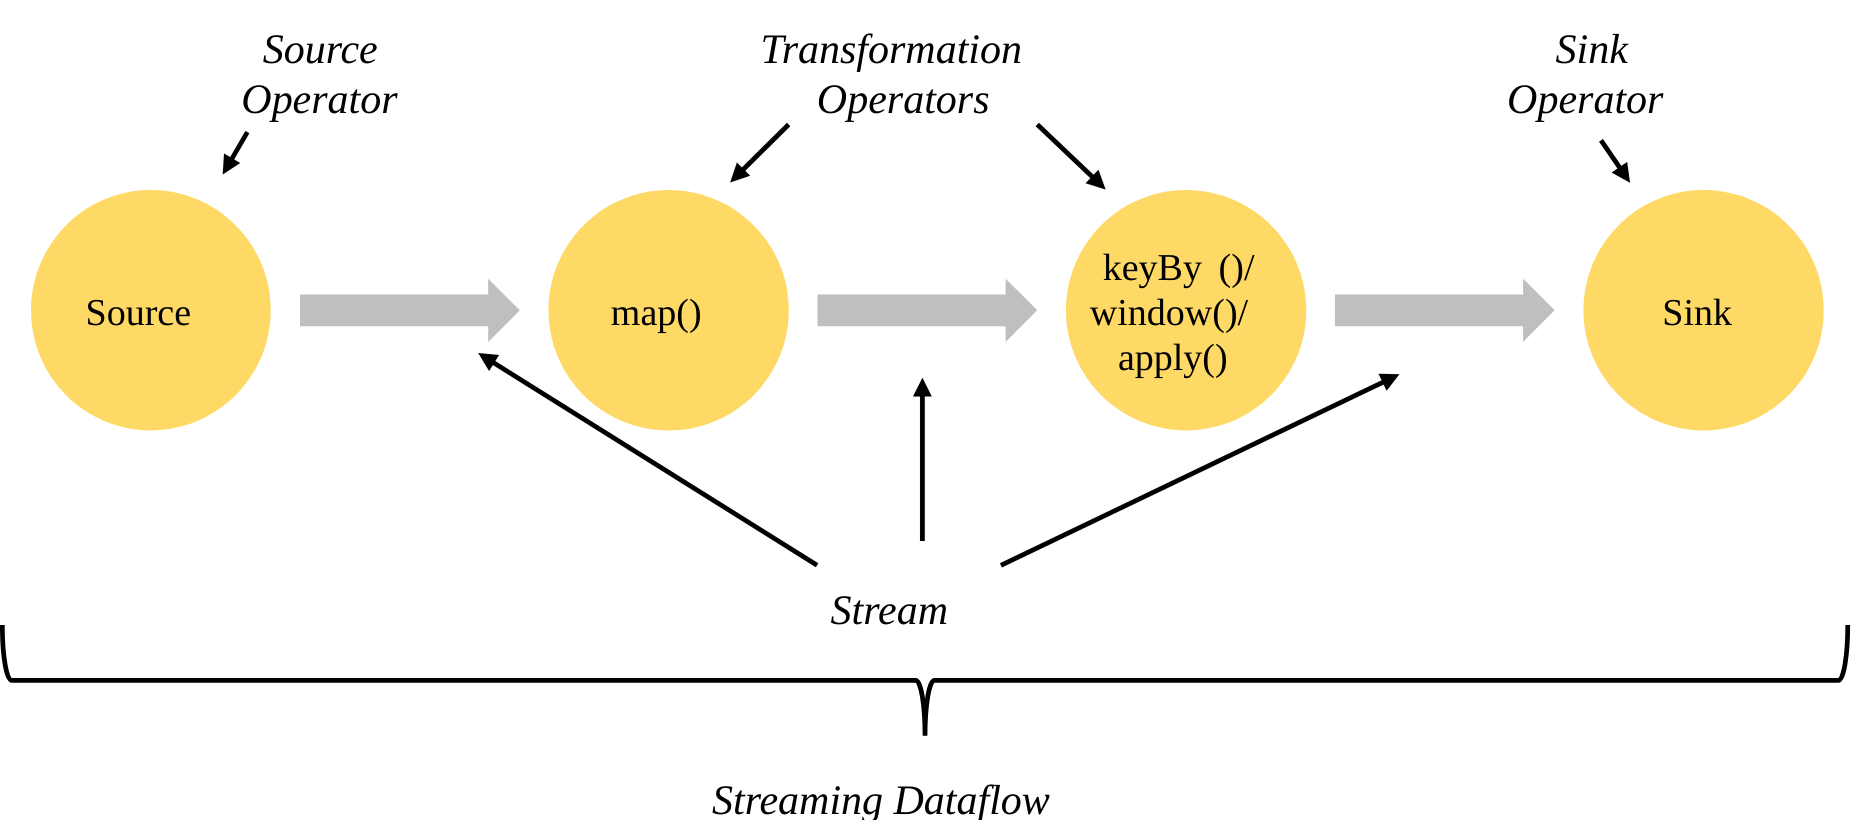
\includegraphics[width=0.9\textwidth]{rw_simpleDataflowInFlink.png}
      \caption{Simple Dataflow in Flink \cite{ApacheFlinkSimpleDataflowFigure}}
      \label{simpleDataflowInFlink}
\end{figure}

Figure \ref{simpleDataflowInFlink} shows a basic program flow. On the left side, it starts with a source. The source is then transferred over a data stream to the first task. The map operation is executed, and the result is sent over a data stream to the next task where the same procedure will start again. The resulting data in this example is the sink, meaning we reached the end of the program. The sink will typically be connected to a database or some other kind of Technology for preserving the data. The most basic option would be to write the sink onto the standard output on the console.

Until now the system can only be distributed by having the different tasks on different physical computers. This distribution process will not suffice when the amount of input data gets too high. To achieve real distribution in the application, each task can be run multiple times as so called subtasks. These subtasks run as a single thread in the JVM and are managed by a task manager. Task Managers connect to a Job Manager which coordinates the distributed execution. The data flow from one subtask to another can either be one to one or as a redistributing data flow. A redistributing data flow is necessary to achieve an even distribution of data at the next subtasks.

\begin{figure}[h!]
    \centering
      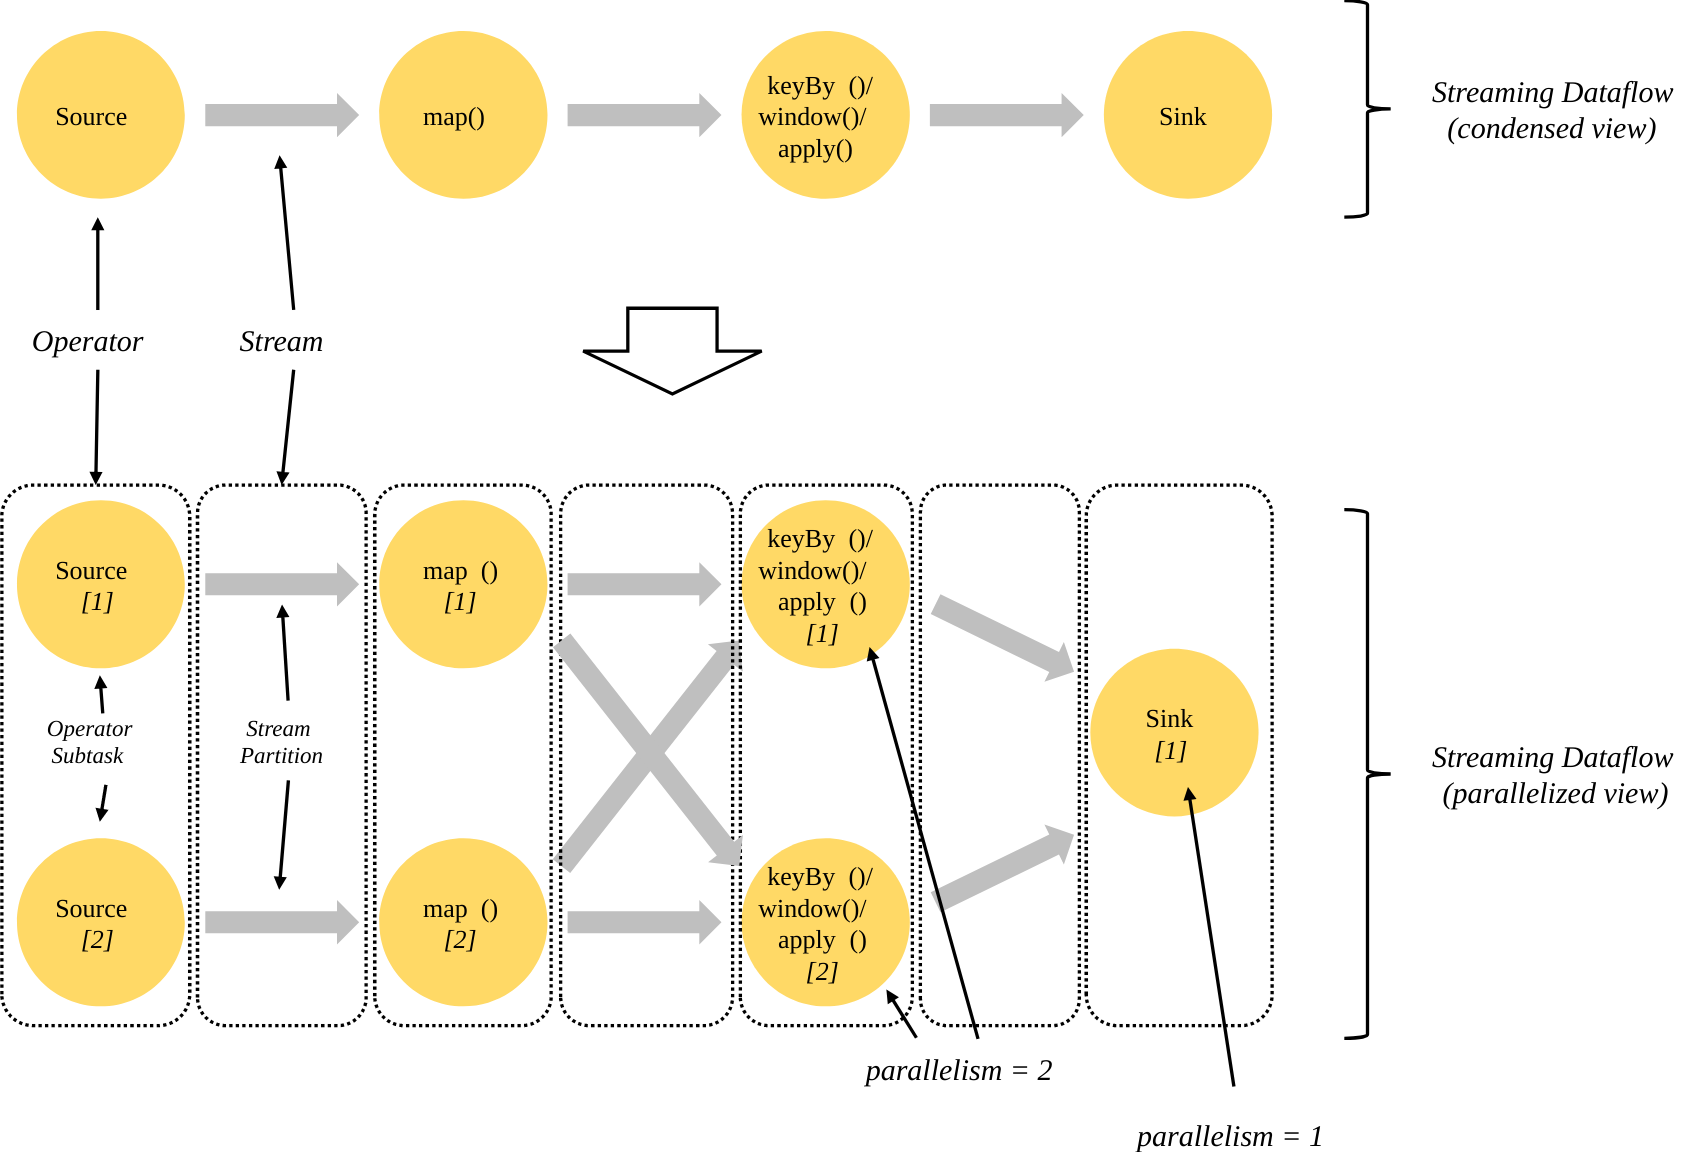
\includegraphics[width=0.9\textwidth]{rw_distributedDataflowInFlink.png}
      \caption{Distributed Dataflow in Flink \cite{ApacheFlinkParallelDataflowFigure}}
      \label{distributedDataflowInFlink}
\end{figure}

Figure \ref{distributedDataflowInFlink} presents the same example as figure \ref{simpleDataflowInFlink} just with the subtasks shown as well. The map task is a vital step in each application as it connects the data from each subtask with each other. It is easily understood by a simple example.
In an application that counts how often each word is in a text, it would only split the text at each space symbol. The redistributing data flow would then create an even distribution in the next node which specifies what to count by (id task) and applies a particular aggregation function to the "apply" operation. The result is then sent to the sink operator. This explanation is a simplification of the actual MapReduce model. For a complete overview see \cite{dean2008mapreduce}.

\subsection{Stream Processing and Batch Processing}

Apache Flink is primarily a stream processing framework, although it can also be used for batch processing. As it makes a big difference in the infrastructure of the framework which process the primary one is, it is important to lay out the differences between the two.

\paragraph{Stream Processing} uses as the names suggest a stream to acquire the data. A stream is an endless sequence of data that can be utilised both as an input and output. As there is no end, it makes it tough to use some algorithms on it. For example, an algorithm that finds the highest number from the input. Flink uses "Windows" to solve this problem. These windows offer a frame for the operations to only use data that was received in each window. Windows can be programmed and provide various ways to define the frame. The simplest way would be just to give a timeframe, but more complex structures could also be built.

\paragraph{Batch Processing} on the other hand has set boundaries, and it is evident how much data is sent and where it ends. To support batch processing as well in the Flink Framework the windows can be programmed to have the same size as the data in the batch. That way even though Flink uses streams it still supports batch processing.

\subsection{Debbugging and Checkpoints}
\label{debuggingAndCheckpoints}
Flink comes with some tools that help the programmer debug his application and help prevent errors stopping the application. This section will highlight what Flink does different or on top of the regular java/scala debugging features.

\subsubsection{Metrics}
\label{metrics}
In a distributed application it can be hard to find out why something is not working properly or why some function performs worse than expected. To help the programmer understand these problems Flink provides metrics, these count or measure throughput on specific points in the application and send this information to a reporter. The reporter provides the information to external applications so that the metrics can be analysed as needed. There are four different metric classes available, a counter that can be in- or decremented, a gauge that can provide the value of a particular variable, a histogram which measures the distribution of long values and lastly a meter that measures the average throughput.

As applications could have a huge number of metrics which would make it very hard to find anything, it is important to have some grouping mechanism. Flink provides scopes to solve this. There are two types of scopes, user-scopes, defined by the user, and system-scopes that hold current information about the system state like the task in which the metric was saved. When a metric is registered, an identifier and a system scope have to be specified, a user-scope can optionally be added.

In addition to the metrics above, Flink automatically collects system information like ram usage, the number of threads, network usage and much more.

\subsubsection{Checkpoints}
\label{checkpoints}

In distributed systems it is quite common that parts of the system crash, this can have many reasons, the incoming data could be formatted wrongly, a data transmission could break away before it is finished, and so forth. Normally the application would log what went wrong and stop or restart the whole application. Depending on how large the application is this could cost a lot of time, flink creates checkpoints which it automatically falls back to if the application crashes. The way these checkpoints work is by periodically injecting barriers at the source. After a task receives a barrier at one of its inputs, it blocks that input until it received a barrier at all of its inputs. Once that happens it takes a snapshot of all the data it received since the last snapshot. This way it is guaranteed that every piece of information is part of a snapshot all the time. To keep these snapshots from taking up too much space on the hard drive flink only stores one snapshot for every task and overrides it with the next. For a more in-depth explanation of this algorithm see: \cite{DBLP:journals/corr/CarboneFEHT15}

As well as these automated checkpoints Flink provides user-created checkpoints called savepoints. These can be set by the user and are not getting deleted everytime a new one is created. They are used to pause the application for example.


\section{Similar work}
\label{similarWork}

Other people did similar work on another framework and distributed systems in general. This section will explore to what conclusions these people came and what can be applied to Flink as well.

\subsection{BigDebug: Debugging Primitives for Interactive Big Data Processing in Spark}

\cite{Gulzar:2016:BDP:2884781.2884813}. The University of California built a debugger for "Apache Spark" which focuses on similar points as this thesis. The motivating intention behind their debugger is to find the cause of the problem easily without having to go through millions of logs, and without stopping the system itself. BigDebug uses five different methods to solve this predicament. This section will not only lay these methods out but also show if they are already present in Flink.

\paragraph{Simulated Breakpoints} are used to debug parts of the application without stopping the running system in every node. This is done by spawning a new process with the same beginning states as the remote one. After that the newly spawned process can be debugged without intervening in the running system.

\paragraph{On-Demand Watchpoints with Guard} are user-defined methods in the system that can be set to inspect the value of a certain variable, check that value and store it in case the value of the variable fails the check. This method can be useful in certain situations for example when checking a variable that is supposed to hold a zip code to see all values that are malformed. This feature can easily be used in the Flink Framework with the use of metrics.

\paragraph{Crash Culprit and Remediation} focuses on two things, first collecting interesting data in case of a program error so that the user can easily find out why the crash happened and secondly avoid rerunning the whole application when a crash happens. These two are grouped together as they are solved together as well. After a crash, the user will get the value that was responsible for the error, for example, the input could have been "23s" instead of 23. The rest of the application will continue to work and once the user corrects the value to "23" the program reruns this task. In Flink, this is partly implemented, as Flink creates automated checkpoints the application will not completely stop when it crashes as it would be in Spark. Flink offers no way to modify values that lead to a program error though.

\paragraph{Forward and Backwards Tracing} is done to make it possible to track where a piece of data came from or where it will end up. This tracing is quite complicated as a piece of data in task X is a sum of all modifications that occurred before that task. The way this is implemented is by tagging each incoming piece of data with a unique identifier and adding all the identifiers that are used to create a new piece of data together. On the other hand, if data is split into multiple pieces, like splitting a sentence into words, every new piece gets a new id, and the relation between the old and the new id is saved. That way a programmer can easily backtrace to where a malfunctioning piece of data originated.

\paragraph{Fine-Grained Latency Alert} is used to identify which records are causing delay. Baseline Spark can already measure the time between each task. BigDebug builds on this feature and extends it by making it available at each operator. This part is quite different in Flink as Flink offers no direct way to apply a metric to each task or operator.

\subsubsection{Conclusion}
BigDebug solves some challenges that a Flink developer has as well. It solves them only in the spark framework and suggests no methodology or procedure for debugging a spark application it just provides some tools for the developer to use.

\subsection{Debugging Distributed Systems}
\label{debuggingDistributedSystems}

\cite{Beschastnikh:2016:DDS:2927299.2940294}: tries to lay out fundamental challenges developer face when building distributed systems and how to solve them.

They give an overview of seven approaches that can help build, validate and debug distributed systems. What follows is a summary of the seven methods.

\paragraph{Testing} is crucial but can only help reveal some errors as testing every piece of the application is impossible.

\paragraph{Model Checking} is a form of testing that automates the testing process somewhat by checking every possible input up to some upper bound in a predefined way. The way the model checker works depends completely on the model checker itself, as there are a lot of different options available. There are for example symbolic model checkers available that explore possible executions mathematically or black-box checkers that just run the application with various inputs. Model checking can be helpful as it can cover much more ground than manually written tests, as well as check parts of the application developers, might not have thought of.

\paragraph{Theorem proving} is a mathematical method of proving that the distributed system is free of defects even before writing a single line of code. It is mostly used for proving that the core of a new application is bug-free before spending lots of time building an application that might not work properly. Amazon is one of the companies using it and released a paper about it as well: \cite{Newcombe:2015:AWS:2749359.2699417}

\paragraph{Record and Replay} is a method for analysing a single execution of the application to gain insight into why an error occurs in a system that has non-deterministic events, as these change every time the program is run even with if the same input values are used.

\paragraph{Tracing} tracing is the method of following data through a system. It has the same goal as Record and Replay have although it is easier to understand what is happening as only a subset of the data is shown.

\paragraph{Log analysis} is a method for debugging black-box systems, but can be used on every application. It is done by applying algorithms to the logs to find bugs that are not easy to spot.

\paragraph{Visulization} is used to make distributed systems more transparent. If a developer has a good visual representation of his work, it is much easier for him to find bad design choices that could lead to bugs.

\subsubsection{Conclusion}
The article provides some basic methods for debugging distributed systems, the analysis of which method is useful is short though.


\typeout{===== File: chapter 4}
\chapter{Debugging Flink Applications}
  
This chapter is the centre part of the thesis. It explains in detail how the method works. It consists of two main sections, the first of which explores in detail what a developer should do while writing the program to minimise the work when debugging. This step is crucial as it is much harder to recreate problems locally as opposed to regular Java applications. The second part focuses on the debugging itself once a developer is informed of an error and has to figure out what is causing it.

\section{Better Developing}
Flink applications are run remotely and without an active user providing input as it is typical for a regular application. Not having a user makes it much harder to recreate the problem as we only have the log files and the stack trace as information. As such it is crucial to have all the information at hand when the program fails, or we notice discrepancies in the resulting data. The only way to make sure that the information is accessible once a problem is reported is to think about what data is necessary for the debugging developer while writing the program. Another issue is that some problems are unique to a distributed environment and won't happen when running on a local host. This section will explain what can be done while writing the program to make the debugging progress much easier.

\subsection{Building Tasks}
The Flink Framework promises a few features that try to set it apart from standard Java applications. These are referenced in \ref{flinkFramework}. The one that sets these applications apart from standard java once while writing the application is the distribution. Applications should be built in a modular way to take full advantage of these features and also make the program easily debuggable.
The development of these tasks should be done using a very similar set of rules as the Unix philosophy states. In fact, Flink modules are not too different to Unix command line tools, they both provide a service while taking an input/output in a predefined way. For the Unix command line, this is the standard output, for Flink programs, these are input and output streams.

\subsubsection{Unix Philosophy}
The Unix philosophy is defined by Doug McIlroy, the inventor of the Unix pipe as follows: \cite{bell1978}
\begin{enumerate}
  \item Make each program do one thing well. To do a new job, build afresh rather than complicate old programs by adding new features.
  \item Expect the output of every program to become the input to another, as yet unknown, program. Don't clutter output with extraneous information. Avoid stringently columnar or binary input formats. Don't insist on interactive input.
  \item Design and build software, even operating systems, to be tried early, ideally within weeks. Don't hesitate to throw away the clumsy parts and rebuild them.
  \item Use tools in preference to unskilled help to lighten a programming task, even if you have to detour to build the tools and expect to throw some of them out after you've finished using them.
\end{enumerate}

Most of the points mentioned here are of some relevance for Flink programming as well. Each task should do one job and do it well. The next paragraph will look into why that is. The second point is necessary by default in Flink, each task has to use the provided streams to work. The third point is equally important if not more important in Flink applications as it is in Unix programs. Always test each Task individually to make sure it works as designed and has no flaws on its own, only then can the whole application work without any problems.

Dividing the program into various modules has a lot of advantages:
\begin{enumerate}
  \item Easier to Develop - It is much simpler to develop a smaller application as it is much harder to lose track of what each piece of code should do. This reduced complexity in return reduces the likelihood of mistakes. Once the program is completed, it results in a more stable program that can be debugged easier.
  \item Better Distribution -  As every Flink task can run on a different computer the smaller the tasks are, the better the Flink Job Manager can distribute the load evenly between the available resources.
  \item Checkpoints are easy to find - Checkpoints are a core piece of Flink technology. It allows the framework not only to jump back and repeat a failed run without having to restart the whole application but also provides information about which state the application is currently in. This is extremely helpful as a lot of Flink applications only end when the program is cancelled by the user.
\end{enumerate}

The modulation of the program not only helps to achieve the advantages of the framework but also supports with debugging later as a lot of the information needed are gathered at the checkpoints.

\subsubsection{Where to split the program}
It should now be understandable that the programs should be divided into multiple tasks, the next question now is how to break the program to get a simple program where there are enough tasks but not too many as too many would lead to the opposite effect we want to achieve.

\paragraph{Why are too many tasks bad?} When there are too many tasks, it gets even more complicated than when everything would be in its task as basically every line of code would be in a different place. Additionally, it wouldn't increase the performance as each task has some initialisation work that would diminish the performance gain achieved by distributing it perfectly.

It makes sense to use the Unix philosophy of having one task do one thing. In most cases there are some obvious choices as in most Flink programs data is modified or analysed each task could be one transformation of the data. It should also be stated that when ever possible the pre-existing transformation functions of the Flink framework should be used. Only in rare situations is it necessary to implement your own data transformation classes. The predefined classes have the advantage of being extensively tested in different conditions thus the risk of data going missing is extremely low.

\subsection{Metrics}
Now that the architecture of the program is done the next question is what metrics to use in which positions to achieve the optimal security.

Once the program architecture is finished, it makes sense to think about what kind of metrics can be used where. Metrics are used to monitor the program without having to debug it and are crucial in notifying the developer if something looks wrong. The first step is figuring out where to use metrics. A good start is to look at the application in the worst possible way; what is the most likely area that an error will occur, after that it makes sense to surround the area with metrics that will catch and log the gathered data. Another great location for metrics is at positions where the through coming data is simple, and metrics can easily be implemented. This should be the case in between tasks. As optimally each task only does one thing it should be easy to check whether the starting and ending assertions are valid.

\subsection{Logging}
Logging in Flink is straightforward and can is used the same as in every other java program that uses log4j. As Flink already provides the necessary libraries to use log4j all a developer has to do is to write the logging config file. Although the logging process itself is the same as every other Java application, it should not be forgotten to use the different log levels that log4j provides. There is a lot of logging happening out of the box just by the Flink process itself. The six logging levels, from highest to lowest are:
\begin{enumerate}
  \item FATAL - the highest logging level, should only be used when the application cannot continue to work because of an unexpected error.
  \item ERROR - whenever an unexpected exception is thrown it should be logged.
  \item WARN - warnings that could lead to errors later on. These are difficult to think of beforehand but if used correctly are very valuable for the debugging developer.
  \item INFO - relevant information like successful database connections and other milestones in the application to let the reader of a log file understand at which point in an application the program currently is.
  \item DEBUG - should be used to record relevant information along the way that could be useful to a programmer when debugging. This could, for example, contain values of variables like database connection strings.
  \item TRACE - is used to let a developer searching for a bug understand the path the application took. Should be logged into a unique log file as it would flood every other one.
\end{enumerate}

\section{The Debugging Process}

There are multiple reasons how an error might be discovered, the most common one being an exception in a log file. Another option is that the end user of the results finds that some of the results are incorrect. Both of these cases require slightly different handling. An excellent way to start the debug process is by using a modified version of the Traffic approach introduced in \ref{aodZeller}.

\subsection{Track the Problem in the database}
Tracking a problem is essential in every development cycle no matter in which language or with what framework and Flink is no exception. It is crucial for every developer to track the status of problems in Flink applications as it helps to minimise work. Along the already mentioned advantages in chapter \ref{aodZellerTrack}, like having an easily accessible database of open problems and knowing which problems are more important than others, tracking the problems of Flink applications offers some other advantages as well.

\begin{enumerate}
  \item Having access to relevant log files.
  \item Knowing how past problems were solved.
  \item What relevant metrics were when the error occurred.
  \item Which subtask of what task manager failed which allows seeing if problems only occur on one machine.
\end{enumerate}

To achieve these advantages the tracking database needs additionally to the already mentioned fields in \ref{aodZellerTrack} a few additional columns. As soon as a problem is experienced the current log files should be saved so that it is easy for the developer to find the relevant lines in the log file even if he starts debugging months later. Secondly, for the same reason, all appropriate metrics should be saved as well.

The resulting columns now are:

\begin{enumerate}
  \item Description
  \item State
  \item Resolution
  \item Assigned Developer
  \item Severity
  \item Link to logs
  \item Steps that were taken to resolve the problem
  \item Relevant metrics
  \item Task manager that was used
\end{enumerate}

\subsection{Reproduce the failure}
Reproducing the problem is probably the most challenging part of debugging Flink applications. As there is no user to report the problem the only help the debugging developer has is information provided by the problem report from the last chapter.

There are two possibilities how a problem is discovered, and both require different steps to reproduce the problem. The first and more difficult one is that an error in the resulting data is discovered without an exception being recorded in the log files. This means that the program is doing something different then what the developer expected when writing it. The second option to discover a problem is by having an exception showing up in the log file.

\subsubsection{Faulty resulting data}
This section will use the word count application as an example program to debug. Notice that the exact implementation of it is irrelevant at this point. The application is a black box as only the incoming, and resulting data are known. To always have the same expected result the following sentence will be used as an input each time: "Hello hello flink flink flink one two". The expected result would be:
\begin{lstlisting}
  hello - 2, flink - 3, one - 1, two - 1
\end{lstlisting}

\paragraph{} The following text explains the process that is used in this case alongside a diagram: \ref{debuggingFaultyData}

\begin{figure}[h!]
    \centering
      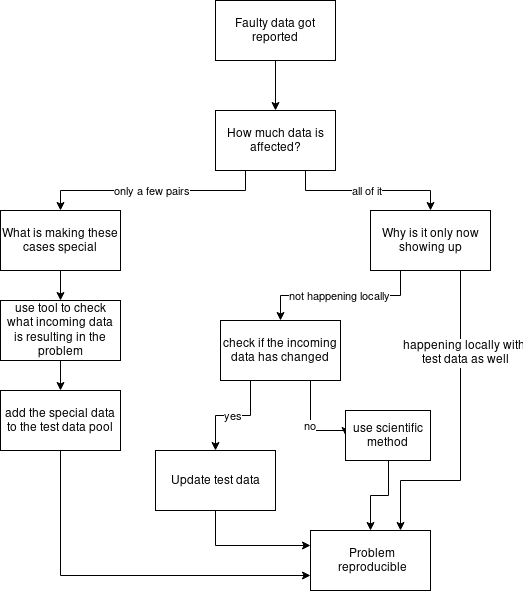
\includegraphics[width=0.9\textwidth]{DebugWithoutException.png}
      \caption{Debbugging faulty data}
      \label{debuggingFaultyData}
\end{figure}

\paragraph{} The first question that has to be answered is
"how much data is affected". Are only a few pieces incorrect or is everything faulty? Imagine the result of the application would be:
\begin{lstlisting}
  hello - 3, flink - 1, one - 1, two - 2
\end{lstlisting}
  Each word has the count of the next word. So this would be considered as the second case "everything is faulty" even though the word "one" has the correct answer. This is important to note as sometimes a fault in a program can still result in a correct result. This first question just differentiates between a few faults and a majority of faults, so the debugging developer has to look at the whole picture and see if the majority of data is corrupt. An example for only a few faults would be:
\begin{lstlisting}
 Hello - 1, hello - 1, flink - 3, one - 1, two - 1
\end{lstlisting}
Here only one additional word was counted ("Hello").
\paragraph{} If the first case is valid (all data is faulty) the next question that should be asked is why the problem is only now showing up. If the problem is observable for almost all the resulting data, surely it should have been noticed while testing the application. In most cases, the problem was either found during testing in which case the problem is already reproducible or was not observable on the local test machine. That means that either the incoming data is different to the local one or that something is being executed differently on the remote network than on the local machine. As Flink is responsible for the distribution and everything is running in a JVM, it is implausible that Flink is to blame. In most cases, the data on the server will differ from the local one. If that can be confirmed the only thing left to do is to update the local test data so that the problem can be reproduced locally.

\paragraph{} The other option was that only some pieces of data were wrong. In that case, the process of reproducing the fault is entirely different. There are two options available. First, figure out what makes the faulty data unique in comparison to the other data. In the word count example, this would be the capital "H" at the beginning of the first "Hello". If this option is successful, the unique case can be added to the test cases, and the reproduction was successful. If on the other hand, the developer can't figure out why the one failing case is different to the others the tool that is written alongside this thesis can be used, it will be explained in detail later on. It can show which incoming data was leading to which result. In the example above it could show that the first "hello" was the result of the original sentence. As there is only one sentence in this example that is not very helpful, but in a more realistic use case, there could be millions of sentences where just a few have capital letters in them. Once the starting sentence is discovered, it can easily be reproduced.

\paragraph{} The last step before moving on to the next section is to make sure that the reproduction works. There is little to no use in finding something in the code that is supposedly the problem only to find out later that the problem is something else.

\paragraph{} The fault should now be reproducible on a local machine as the affecting test data was found. The only fault that remains are problems that only occur on the remote network and are not happening because of differing incoming data. In almost all cases the root of these problems is either incompatible Flink components or network issues. So before starting a more complex search for the problem the developer should check the Flink documentation if all used components, like data sources, the chosen backend etc. are compatible with each other. Furthermore it makes sense to check if all of the running systems can send packages to each other and the database as firewalls and other network related issues could be the issue. If none of these are quickly found it is recommended to use the scientific method described in: \ref{aodZellerIsolateDefect}

\subsubsection{Exception in log file}
The most common way to discover a failure in a program is by discovering an exception. It makes no difference if this exception was found in a log file or directly in the developer's console. The steps that are necessary to reproduce these errors are often easier as well.

\begin{enumerate}
  \item What kind of error was thrown? - The developer should always keep in mind what type of exception was thrown as it is much easier to find the origin of the failure when knowing what to look for.
  \item Where was the failure thrown? - This information is the starting point for the search of how to reproduce the failure. It is included in the stack trace of the exception so it shouldn't be a problem finding it.
  \item Isolate the conditions in the method - Knowing under which conditions the failure occurs is crucial. Without this information, it is almost impossible to reproduce the failure reliably as only a few errors occur under all circumstances. The developer should start by just focusing on the method the exception is thrown in and finding the conditions by looking at the "if statements" that precedent the line in question. Note in which state each variable has to be for the exception to be thrown. This can include the variable that is throwing the exception as well. In most cases, the developer should now already have a pretty good idea as to when the error occurs and if that is the case can skip the next step to save time.
  \item Repeat the same step for the method - Once it is understood in which conditions the failure occurs in the given method, the developer has to find out in which cases the method is being called with the conditions that were deducted in the last step. This can be done by repeating the step above only for the line where the method was called, which is included in the stack trace of the exception as well. This step has to be repeated until the start point of the application has been reached. At this point, the developer should have a good understanding when the exception is thrown and should be able to reproduce it.
\end{enumerate}

\subsubsection{Conclusion}
In most cases, the developer should have no problem reproducing the error easily without going to much in depth into the steps presented in this chapter. Although these steps help to guide a developer that might not even be deeply familiar with the code through the process with ease sometimes problems occur that can not be found using these steps as they are too unique and would not appear for anybody else. If a developer stumbles over such a problem, it is suggested to apply the same method that is explained in \ref{aodZellerIsolateDefect} by creating a hypothesis checking the outcome and repeating the process until the failure can be reproduced.

\subsection{Automate and simplify the test case}
In comparison to typical Java applications where automated testing can be quite tricky as a graphical user interface, and user interaction is involved, automating the test cases for Flink applications is quite easy assuming that the problem is reproducible on a local machine. All that the developer has to do is take the result of the last section and write a test with the specific start parameters. The "Traffic Approach" also suggests simplifying the test case to be as easy to implement as possible so that only the error and nothing else gets checked. This can be useful to make it easier to help spot the problem in the code later on but is not needed for Flink applications. For example, if the word count application were to crash on "-" characters and the input test case would be an entire book page of words it makes it harder later on to find the actual character that is causing the fault but makes it easier to create the test case. As understanding the problem and simplifying the test case is mostly the same it makes sense to leave the test case long and rebuild it once the failure is understood. This way if the same mistake gets built into the code again it is easily spottable as the test case already has a descriptive name, description as well as a ticket number associated with it. Another developer could then easily reproduce the steps that were taken to solve the problem the last time.

\subsection{Find possible infection origins}
This step in the debugging process is just a collection of possible points to start the debug process from. It is always possible to change this point later if the chosen point turns out not to be the origin of the infection. Flink applications are very different to other Java applications in this section. Flink uses a special way to write applications that makes it possible to run on multiple machines without having to specify how and more importantly which information are transfered between different machines. Because of this complication, code that is written in Flink is being executed before a single line piece of information is read. At the end of each application is an execute statement which then starts the application. When debugging the code written by the developer with a debugger the only information that can be gathered is whether or not flink can successfully build the execution tree or not. The only relevant information this provides to the developer is that all checks that Flink itselfs runs before executing are true. At the time of writing this thesis (Flink 1.5) it ensures successful connections to the databases or other data stores used by the application and  compatibality of the used datasources and backend. As an example if a backend that supports snapshots is chosen, Flink will check if the first datasource supports rollbacks as that is a requirement of snapshots. Other problems like incompatible datatypes can still occur afterwards.

this section includes the next step of the traffic approach as Flink applications are strucured in a way that makes it very easy to find the possible origins with the information given here. To make it even easier the word count example from the beginning of the thesis is used again, this time as an actual Flink application:

\lstinputlisting[language=Java]{WordCountFlink.java}

What this program does is the same as the earlier word count example, it counts how often each word is in a specified input. As this is written in the Flink framework it uses streams to store the data and tranformation methods to connect the streams in a way that splits and then counts the words. The first stream is used to gather the incoming data from an apache kafka cluster (Line 5). The data stream is called "text" and is used in the next stream as a source (Line 8). This data stream is called "counts" and is doing the actual work of the program. It uses a flat map function to split the string at each space symbol and uses the newly created "words" to add them to a new String, Integer tuple. Flink then simply adds all these tuples that have the same key together and adds up the Integers. This can be done as the whole transformation method is an extension of the flatMap method that is eventually adding all created tuples together.

\subsubsection{Exception before application is executed}
The first case that we are going to look at is that the application throws an exeption before it is being executed. This is the case if any of the lines before the execute line appear in the stack trace. In our example the execute line is line 11. so the a possible exception that would fit in this category would be:

\begin{lstlisting}
java.net.ConnectException: Connection refused (Connection refused)
  at com.jakobjoachim.WordCountFlink
  $WordCountFlink.main(WordCountFlink.java:5)
\end{lstlisting}

As stated above connection problems are not the only issues that can cause an exception before the execute line is reached. It is also possible for some of the Flink components to be incompatible with others. No matter which of these two is the case the procedure is the same. As the failure happens before any of the Flink specific issues are encountered the method described in the standard "Traffic Approach" \ref{aodZellerInfectionOrigins} is enough to find the root of the problem. This means going to the specified line in the stack trace and checking if the line could be responsible. As Flink applications are only a set of transformations on datastreams this search is relativly easy as it is most probably found either at one of the transformations or at the inital connect to the database.

Because of how Flink works in this step there are only two possible roots for an issue in this category. Either the line that throws the exception or the other side. In case of Flink component issues this means the line that sets up the datastream or environment that is being used in the line that is throwing the exception. Because of this it is not necessary to follow the next step of the Traffic Approach (Focus on the most likely origins).

\subsubsection{Exception in a transformation method}
Another possible case is that an exception was thrown while the application is running. On contaray to exceptions that occur in the datastreams and will not show the line written by the developer in the stack trace, exceptions in transformation methods will show up as the source in the stack trace. If we look at line 23 and 24 in the example application we will see that an error is thrown whenever the word "test" is read. Of course this is set up to throw an error and a real application would be more likely to throw a nullpointer ecxeption or similar when tranforming the data (line 27). When "test" used as part of the input the following stack trace is thrown:

\begin{lstlisting}
java.lang.Exception
	at com.jakobjoachim.WordCountFlink
    $LineSplitter.flatMap(WordCountFlink.java:24)
	at com.jakobjoachim.WordCountFlink
    $LineSplitter.flatMap(WordCountFlink.java:14)
	at org.apache.flink.streaming.api.operators.StreamFlatMap
    .processElement(StreamFlatMap.java:50)
	at org.apache.flink.streaming.runtime.tasks
    .OperatorChain$CopyingChainingOutput
    .pushToOperator(OperatorChain.java:549)
  ...
\end{lstlisting}

The only lines that are part of our code in this stack trace are the lines in the flatMap method. The stack trace does not show which of our datastreams called the method. This is because the datastream was converted to a flink internal datastream before the application was run. As such the next step is to find out which of our datastreams called the transformation method in question. Possible infection origins are now:

\begin{itemize}
  \item Bug in the code of the flatMap.
  \item Bug in transfer to the data stream that called the flatMap method.
  \item Bug in any data stream or transformation of data streams before that.
\end{itemize}

Failure in transfers between data streams are highly unlikely when the program can be reproduced localy as any incompatible data types and components are already checked. Although this is only true if Java generics were used with all appropriate variables. These possible infection origins are enough to uses as a basis for the next section called "Isolate the defect in the chain" \ref{mdfIsolateInfection}.

\subsubsection{Exception in internal Flink code}
The last possible location to throw an exception is the internal FLink code itself. This can have a lot of possible reasons and the least amount of helpful information in the stack trace. One possible reason could be a timeout while sending data from one machine to the other. The exception will show that some sort of network timeout was the cause but there is not much else in the stack trace that can help the developer narrow down the search. This is why logging correctly is crucial in this section as the most relevant pieces of information are which data stream was responsible. The log file contains such information and can be seen either directly by reading the log or by using the Flink web ui if it is used.

\paragraph{} We should now know which datastream is causing the exception but possibly, depending on the thrown exception, not why. This step of the debugging process requires a lot of understanding of how Flink and the program that is being debuged works. There are a lot of different reasons why an internal exception might be thrown. The good news is that it is very unlikely that the fault is somewhere else in the code and that the data stream that is throwing the exception is working fine. In almost all cases the it is either the data stream throwing the exception or the transfer to that data stream. Because of that we can use the datastream line as our infection root for now.

\subsubsection{No Exception but resulting data is faulty}
if there is no failure and the resulting data is wrong, the developer can use the line where the false data got stored as the "exception throwing line". At that moment the failure is already present in the application so the line can serve the same way an exception would. If the program is too complex to overview how it got to that point a stack trace can be printed to the console by adding the following line (remove this afterwards):
\begin{lstlisting}
 System.out.println(new Throwable().getStackTrace())
\end{lstlisting}

\paragraph{Brief introduction to the Flink Backtracking tool}
\label{mdfBriefIntroTool}

To narrow down the search to a line that might actually be responsible the developer can use the tool that was designed alongside this thesis and is explained in detail in chapter \ref{TODO}. The tool allows the developer to see the content of the data streams in real time and also shows the relation between the data and multiple data streams. This is done by using  the Flink watchpoint mechanism to split the inputs into groups. In the Word Count example which has two data streams this would result to the following with an example input of "this is a test this is a test is this a test?":

\begin{itemize}
  \item \textbf{Data stream 1 - Watchpoint 2321:} "this is a find this is a find", \textbf{Watchpoint 2346:} "is this a find?"
  \item \textbf{Data stream 2 - Watchpoint 2321:} "this - 2, is - 2, a - 2, find - 2", \textbf{Watchpoint 2346:} "is - 3, this - 3, a - 3, find? - 1"
\end{itemize}

If this was part of a bigger input in a more complex program the developer might not have seen directly why the word "find" was only counted two times when it was cleary in the input three times. Because he now has a direct overview of what data transformation happend at which point he can easily spot at which transformation the failure is firstly observable and use that as the infection origin.

\subsection{Isolate the infection in the chain}
\label{mdfIsolateInfection}
Now that the root of the infection was narrowed down to a few possible lines of code it is time to isolate these lines to see if they are in fact the cause of the issue or merley another infected line.

It is yet again necessary to split this section into multiple parts depending on which kind of infection is present. We can skip this chapter altogether for exceptions before the the applicaton is executed because we already know for sure which line is causing the issue and only have to correct the defect.

\subsubsection{Exception in a transformation method}
Isolating the transformation or data stream that is causing the issue can be done by firstly looking at the exception it self. It might be obvious that the the line showing up in the stack trace is resposible or that such an exception should never be allowed to crash the program. Another important step while finding the issue is to make sure that exceptions that crash the application are only doing so when there is no other way. It might be possible to log the exception and ignore that part of the input as long as the program can continue running. Most Flink applications run on huge server farms where each hour costs the company a lot of money so full applicaton crashes should be minimized.

If the issue is not obvious it makes sense to use the tool that was developed alongside this thesis that was already briefly mentioned earlier: \ref{mdfBriefIntroTool}. In the same way that the tool is useful when finding corrupted data in the streams it can help us here to gain a deeper understanding into what is happening in each stream. Together whith the reproducable test and tool we should see how the data that is causign the issue got to the transformation in question. We can then correct the defect as we isolated the faulty transformation.

\subsubsection{Exception in internal Flink code}
No matter where in the Flink internal code an exception is thrown we can use the information from the log file to find out which data stream was resposible. Then run the program a few more times to make sure the exception is always thrown at the same data stream. The next step is to make sure that the incoming data is the correct and there is no error present beforehand. Also it makes sense to check if the incoming data can be manually added to the test case of the transformation at the faulty data stream. If that also works we know that the root of the infection is in fact the data stream. This is enough to correct the defect. If, on the other hand, one of these checks failed we have to go back a few steps and include the option that a transformation might be faulty depending on which of these checks failed. If the the exception is thrown at different places all the time it makes sense to google the exception to make sure that it is not a common problem with Flink. If it is not use the scientific method to narrow down the search until the root cause is found.

\subsubsection{No Exception but resulting data is faulty}
We now have a specific location at which the data gets corrupted. To solve the issue the developer has to look at the transformation method that is used by the data stream. The method can then be debugged on its own be writing a unit test for the method and using the normal Java debugger with breakpoints to exactly see what is happening. To make matters even easier in case the method is very complex the developer should still use the same method described in \ref{TODO}

\subsection{Correct the defect}
With all the information gained by the previous steps we now know where the issue originates from and we can fix the issue. There are a few possibilities:

\begin{enumerate}
  \item[mdfCorrectTransformation] Transformation method Faulty
  \item[mdfCorrectNetwork] Network issues
  \item[mdfCorrectDataStreams] Data streams are causing the issue
\end{enumerate}

\subsubsection{Transformation method faulty}
\label{mdfCorrectTransformation}
The first step in correcting a failure in a transformation method is to make sure that the unit test checking that method is updated so that the same error can't happen again. Another important thing to rhink about is if such an error would happen again would it be better if the application didn't crash but instead log the error as critical log level and continue on? This could save the company a lot of money in computing cost. It is a good rule of thump that Flink applications should never crash once they are deployed.

\paragraph{Correting the defect} Now that all the prerequirements are done, it is time to actually start correcting the defect. Using the newly written test case and the java debugger we can go through step by step and see at which point the failure appears. Most of this task should already been done by the steps beforehand. If for whatever reason the exact root of the failure could not yet been located, we can use the scientific method to further narrow down the possiblities until the root is found.

\subsubsection{Network issues}
\label{mdfCorrectNetwork}
Connection issues are quite common, following these steps should result in a working connection:
\begin{enumerate}
  \item Network issues: Both firewalls need to be setup correctly to allow packets through. This can be checked by starting a simple tcp connection between the two systems with Netcat or a similar program.
  \item Configuration issues: The database has to accept incoming connection requests from the corresponding ip range. This has to be configured in the database settings and varies between different databases.
  \item Flink database adapter: Flink has to support the chosen database or a database connector has to be written. Consult the Flink documentation and check if the adapter version is compatible with the Flink version.
  \item Configuration issue: The IP address that is used in Flink could be wrong or the username and password for the connection.
\end{enumerate}

\subsubsection{Data streams are incompatible}
\label{mdfCorrectDataStreams}
There are two possible reasons why data streams would casue problems. Either they are not compatible, or the data that is transfered in them isn't. Another option that should already have been ruled out is a network issue \ref{mdfCorrectNetwork}. Lastly data could arive at the latter data stream in the wrong order. This is only relevant for some applications as most Flink applications, like the word count example, do not care in which order the input arives.
\begin{itemize}
  \item \textbf{Data types} - The developer should make sure that Java generics are used at every appropriate location. This ensures compatibility of the data types because the java compiler checks them.
  \item \textbf{Data streams not compatible} - The developer should check the documentation of each of the used data stream features to make sure both are compatible. Lastly if that failed also check that the Backend is compatible in the same way.
  \item \textbf{Data in wrong order} - TODO
\end{itemize}

\subsubsection{Conclusion}
Although fixing the defect is the reason the whole debugging process was started it is not the end. As explained in the \ref{aodZellerCorrectDefect} other questions need to be answered before the developer can move on to something else.

\paragraph{} Alongside the already mentioned tasks a Flink developer should also think about the following steps:
\begin{enumerate}
  \item If there was no exception thrown and the failure was purely faulty data, it is not enough to have a test case that makes sure that the same error gets reported again, but the developer should also add a check into the program that throws an exception. This is important as it is crucial that faulty data can't be generated by the program.
  \item If the test case was not simplified now is the time to fix that. The developer should shorten the input to the bare minimum that would produce the failure, rename the test case accordingly and add the ticket number as a comment to the test case.
\end{enumerate}


\typeout{===== File: chapter 5}
\chapter{Flink Backtracker}
\label{flinkBacktracker}
  This chapter will explain in detail how the Flink Backtracking tool written along side this thesis works and how it is used. It is composed of two parts, the frontend part that shows the results in the IDE and the backend part that has to be included in the project that sends the information to the frontend. This chapter is thus split into multiple paths:
\begin{enumerate}
  \item[\ref{fbManual}] User manual
  \item[\ref{fbBackend}] Backend architecture
  \item[\ref{fbFrontend}] Frontend architecture
  \item[\ref{fbState}] State of the program
\end{enumerate}

\section{User manual}
\label{fbManual}

\paragraph{Introduction to the Flink Backtracking Tool}
The Flink Backtracking Tool allows the user to see what data was read at each data stream and what data lead to the result at the next data stream. The Flink Watchpoint mechanism is used which injects a barrier with an indentifier every so often. The data between each of these barriers at each data stream is thus the result of the data between the same barriers plus the transformation of the previous data stream. Thus the exact result of each data stream can be seen which is not possible with step by step debugging.

\paragraph{Prerequirements} There are a few prerequirements that have to be met to make the progrgam work appropriatly. First and foremost it has to be a Flink application as it can only track Flink data streams. Also because it is using the watchpoint mechanism of Flink all requiremts that go along with that have to be met. This means each datastream has to support rolling back data in cases of a failure. Because of this requirement it is currently only possible to use data that comes from some sort of big data storage. In the following examples Apache Kafka will be used.

Using the program is an easy process. The "FlinkBacktracking.jar" has to be integrated into the Flink application that is being developed and the "FlinkBacktrackingIntelliJPlugin.jar" has to be activated in IntelliJ to see the results of the Tool. There is only one line needed to enable the tool itself, although checkpointing still has to be enabled manually:

\begin{lstlisting}[caption={How to use the Backtracker}]
env.setStreamTimeCharacteristic(TimeCharacteristic.EventTime);
env.enableCheckpointing(1000);
FlinkBacktrack backtracker = new FlinkBacktrack(env);
\end{lstlisting}

Where "env" is the Execution Environment. Any number of watchpoint behavior is possible, in this example it is set to inject a berrier after the specified amount of time. Once the Backtracker is initilised it can be used by adding each datastream that the developer wants to be watched to the tool. This is done in the following way:

\begin{lstlisting}
backtracker.track(dataStream, "Transition name");
\end{lstlisting}

Where "dataStream" is the dataStream that should be tracked and "Transition name" is an arbitrary name that is used to show the results under. This step has to be repeated for each data stream that should be watched. Once these steps are done the developer can open the "Flink Backtracking View" by clicking on the button with the same name on the lower right side of IntelliJ and start the application.

\subsection{Debugging a Program with the Backtracker}
Once the plugin has been configured the application can be started. Each piece of data that is being processed by the application will show up in the "Flink Backtracker" tab in IntelliJ as well. The first tabs that are shown are the different data streams. Each watched data stream has its own tab. Each of these tabs contains a list of watch points that passed since the program was started and each of these includes the data that was processed by that data stream at the time of the watchpoint.

\begin{figure}[h!]
    \centering
      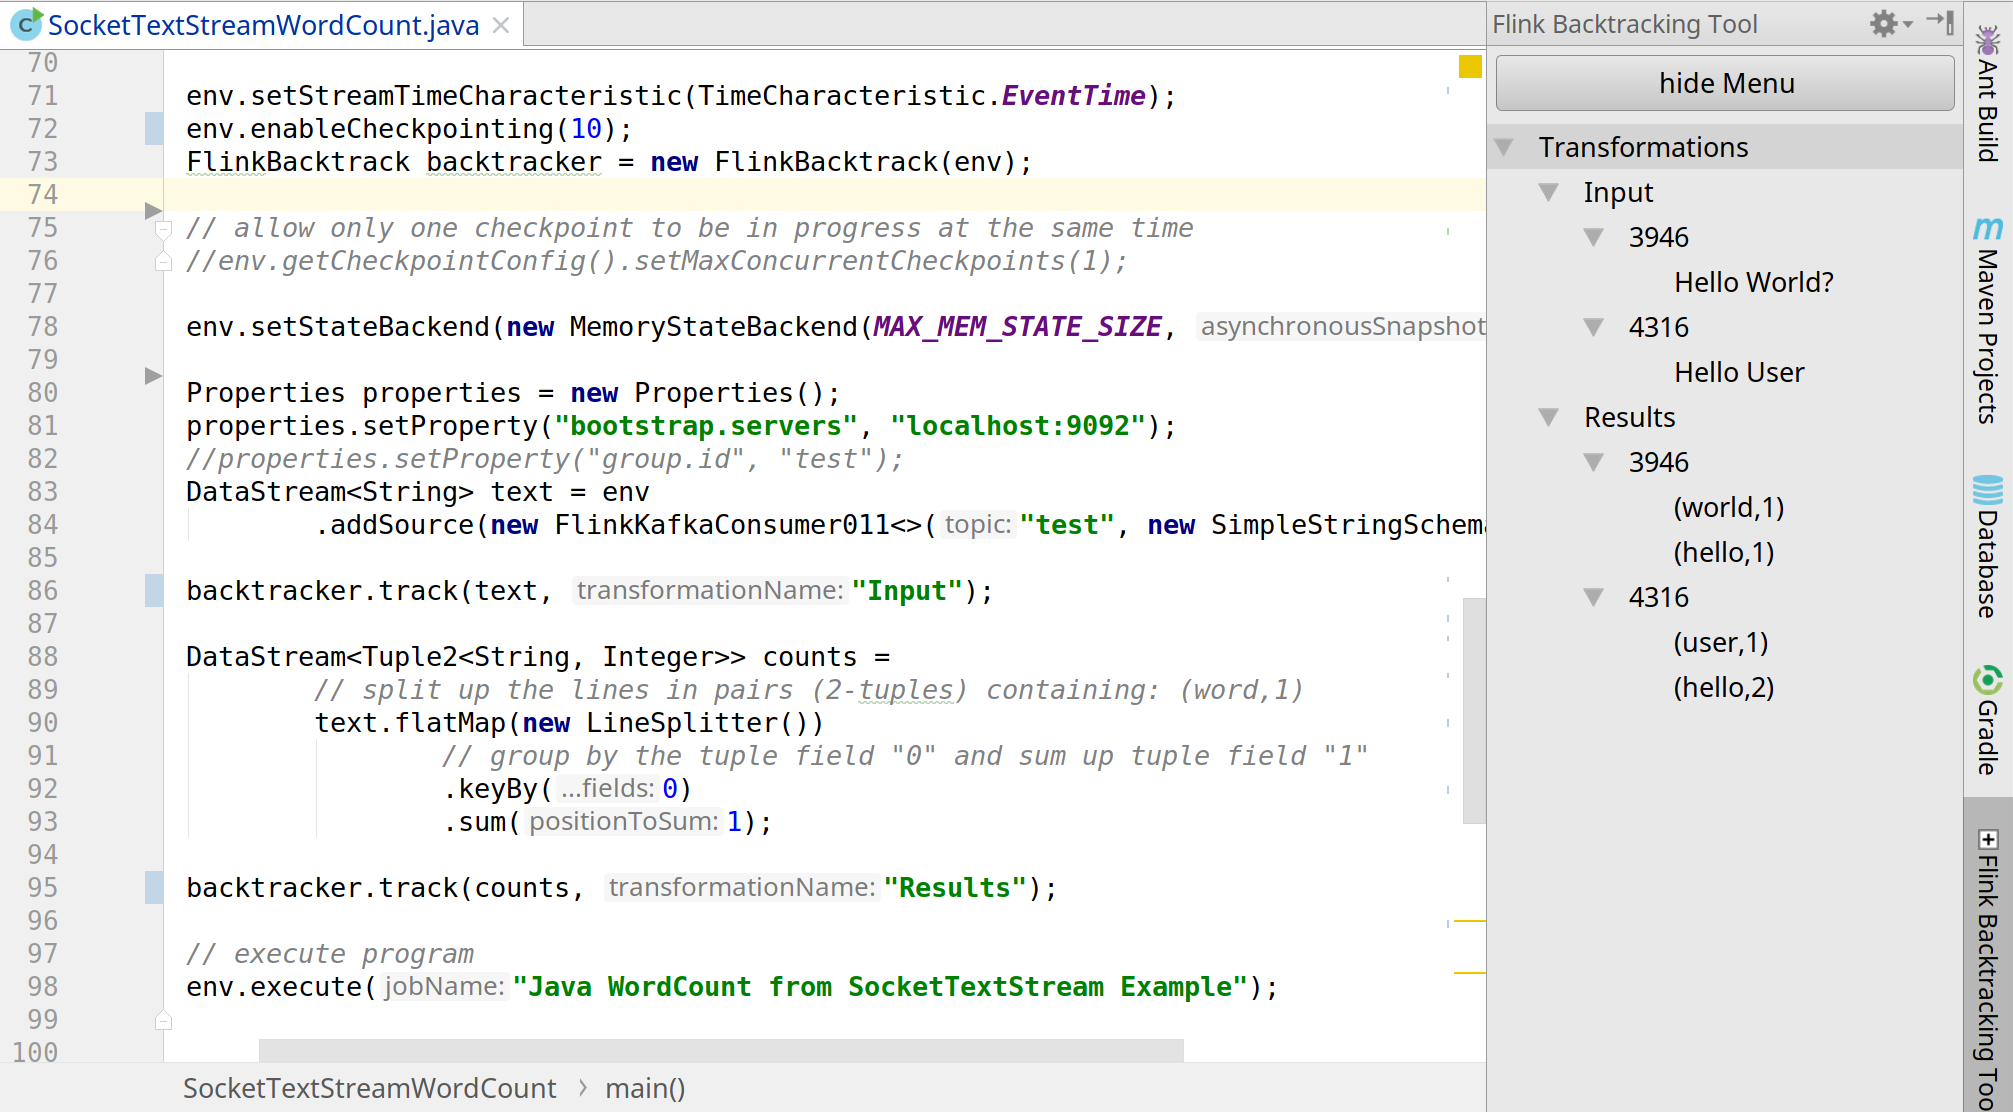
\includegraphics[width=0.9\textwidth]{FlinkBacktrackerIntelliJPluginExample.png}
      \caption{Backtracking Example}
      \label{flinkBacktrackingExample}
\end{figure}

\paragraph{} The example \ref{flinkBacktrackingExample} shows a good use-case for the tool. The developer can easily see that the input of the program was successfully received by the first data stream. He can also see that the application is removing special characters and converting all capital letters. Because the content of the second data stream (result) is not only depending on the data stream that came before (input) but also on all the data that was processed by the stream previously. Thus the "hello,2" in the result transition at watchpoint 4316.

\section{Backend architecture}
\label{fbBackend}
The Backend is composed of two parts one is the function that is collecting the data and sending it to the frontend the other is main class that is used to set up the function in the correct way to ensure that the function can gather all the neccesary information.

\paragraph{} The following example (\ref{dataFlowNoBacktracker}) helps to underline how the Flink application is set up so that the data can be sent to the frontend.

\begin{figure}[h!]
    \centering
      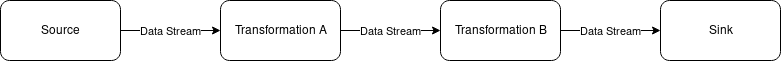
\includegraphics[width=0.9\textwidth]{DataFlowNoBacktracker.png}
      \caption{Dataflow without the Backtracker}}
      \label{dataFlowNoBacktracker}
\end{figure}

\ref{dataFlowNoBacktracker} is a simple application with 2 transformations much like the Word Count application used throughout this thesis. The first transition is reading the input and the second is modifying it. At each transition we split the data stream and send an exact copy to another transformation that is part of the Backtracker that sends it to the front end. That means that with the Backtracker enabled the earlier diagramm now looks like this: \ref{dataFlowWithBacktracker}

\begin{figure}[h!]
    \centering
      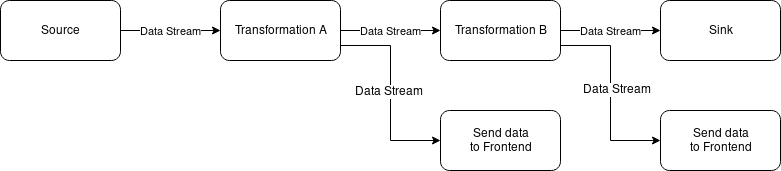
\includegraphics[width=0.9\textwidth]{DataFlowWithBacktracker.png}
      \caption{Dataflow with the Backtracker enabled}
      \label{dataFlowWithBacktracker}
\end{figure}

This ensures that the data is sent to the frontend but fails to show which pieces of information are related to each other. Because of that it is necessary to add watchpoints to the system. The way that Flink handles watchpoints is simple: They are injected at the beginning of the application as part of the data stream, and each time a transformation receives one it injects the same one back at its output at the same position. Each watchpoint is identified by a unique number and is used as a grouping method in this tool. Flink does not allow the current checkpoint to be read out because there can be multiple active at the same time in different parts of the application. The only way to get the current checkpoint for a given transition is by saving the last checkpoint that was read by the transition. The snapshotState method is called by the Task Manager each time a new watchpoint is registered. The following line then saves the checkpointId as a field of the class so that the most recent watermark is always available:

\begin{lstlisting}[caption={Save Watermark}]
@Override
public void snapshotState(FunctionSnapshotContext context)
throws Exception {
  currentWatermark = context.getCheckpointId();
}
\end{lstlisting}

When sending messages to the frontend the current watchpoint can then be added.

\paragraph{Sending Data}

Another important step along the way is sending the data to the frontend. This is done by astablishing a socket connection to the frontend (the frontend is the server) and sending Java objects over it.

\section{Frontend architecture}
\label{fbFrontend}
The frontend architecture is pretty straigt forward. A view is created and populated with a tree view together with a socket server that is avaiting messages from clients. Once it recieves a message it checks if the transformation and/or watchpoint is already present in the tree and fills the data to the correct location. The server can never stop intelliJ from working as it is running in a seperate thread, thus ensuring that any problems with the connection are isolated.


\section{State of the program}
\label{fbState}
The backtracker tool is in a working state, that being said it is not tested in the most vigorues way possible and there are still a few features that would really enhance the usability like being able to save the results.

\paragraph{Saving results}
At the moment the only way the data can be displayed is by using the IntelliJ plugin. Because the messages are sent by the internal transformation a second transformation could be written that instead of sending the data to the IntelliJ plugin saves it in a data base or logs it to a file. When creating the Backtracker a second constructor was needed to specify which Backend function to use.

\paragraph{Better UI}
The UI still lacks a few features that would drasticly increase the ease of the program like clearing old results or saving the tree directly from there.


\typeout{===== File: chapter 6}
\chapter{Conclusion and Outlook}
  Summing up all the pieces, this thesis provided a methodolgy for debugging Flink applications. The basic procedure of a Flink application was discussed and the pitfalls of writing such programs marked, along the thesis a sample word count application was used to picturize the methods. A backtracking tool was written that provides the developer with more information then are normally availble.

Something about only the data stream api was covered


%% appendix if used
%%\appendix
%%\typeout{===== File: appendix}
%%\include{appendix}

% bibliography and other stuff
\backmatter

\typeout{===== Section: literature}
%% read the documentation for customizing the style
\bibliographystyle{dinat}
\bibliography{thesis}

\typeout{===== Section: nomenclature}
%% uncomment if a TOC entry is needed
%%\addcontentsline{toc}{chapter}{Glossar}
\renewcommand{\nomname}{Glossar}
\clearpage
\markboth{\nomname}{\nomname} %% see nomencl doc, page 9, section 4.1
\printnomenclature

%% index
\typeout{===== Section: index}
\printindex

\HAWasurency

\end{document}
